\documentclass[11pt]{article}
\usepackage{fullpage,lipsum,amsmath,amsfonts,amssymb,graphicx, subcaption,enumitem,mathtools,float}
\font\titlefont=cmr12 at 20pt
\font\subtitlefont=cmr12 at 17pt

\title{%
  \titlefont{COMS W4701: Artificial Intelligence, Spring 2025} \\
\subtitlefont{Homework \#3}} %replace \# with number
\author{Peter Driscoll (pvd2112)} %replace with name & uni

\begin{document}
\maketitle

%Problem 1
\section*{Problem 1}

%Subsection 1.a
\subsection*{1.a)}
\begin{figure}[H]
\centering
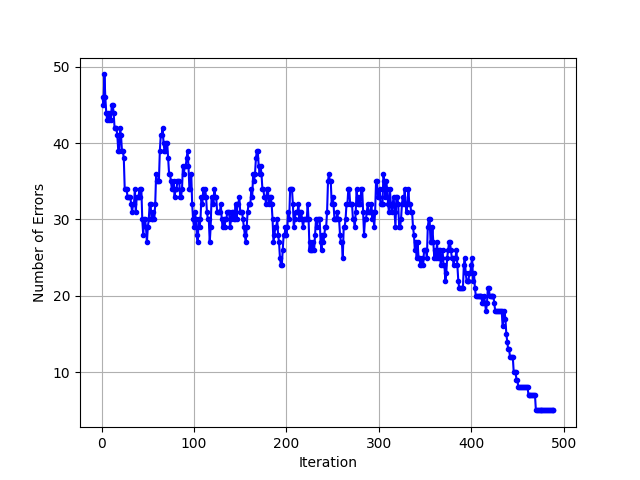
\includegraphics[width=0.7\textwidth]{images/Figure_1.jpg}
\vspace{1em}

\caption{Mini-Blackjack State Transition Diagram}
\label{fig:1}
\end{figure}

%Subsection 1.b
\subsection*{1.b)}
The optimal action for states 5 and 6 is the $stop$ action. The stop action at these states yields $V^*(\text{stop}) = 5$ and $V^*(\text{stop}) = 6$, respectively.
This is because the draw action from these states will always result in a sum greater than 6, which yields $V^*(\text{done}) = 0$.

\pagebreak

\begin{table}[h]
\centering
\renewcommand{\arraystretch}{1.5} % Increases row height for better readability
\caption{Optimal Actions and Values for Remaining States}
\label{tab:optimal_values}
\vspace{1em}

\begin{tabular}{c|l}
\hline
\textbf{State} & \textbf{Optimal Value Calculation} \\
\hline
4 &
$V(4) = \max \left\{  \frac{1}{3} \cdot V(6), 4 \right\}
\Rightarrow \max \left\{ 2 , 4  \right\}
\Rightarrow 4$ \\
\hline

3 &
$V(3) = \max \left\{  \frac{1}{3} \cdot (V(5) + V(6)), 3 \right\}
\Rightarrow \max \left\{ \frac{11}{3} , 3  \right\}
\Rightarrow \frac{11}{3}$ \\
\hline

2 &
$V(2) = \max \left\{  \frac{1}{3} \cdot (V(4) + V(5) + V(6)), 2 \right\}
\Rightarrow \max \left\{ 5 , 2  \right\}
\Rightarrow 5$ \\
\hline

0 &
$V(0) = \max \left\{ \frac{1}{3} V(2) + \frac{1}{3} V(3) + \frac{1}{3} V(4) , 0  \right\} \Rightarrow \frac{38}{9}$ \\
\hline
\end{tabular}
\end{table}

\vspace{1em}

\begin{table}[h]
\centering
\renewcommand{\arraystretch}{1.3} % Adjust row height for readability
\caption{Summary Optimal Actions and Values} % This caption will make it "Table 2"
\label{tab:summary_optimal_values} % You can reference it in the text with \ref{tab:optimal_values}
\[
\begin{array}{c|c|c}
  \text{State} & \pi^*_{t=1}(\text{state})
  & V^*(\text{state}) \\ \hline
  0 & \text{draw} & \frac{32}{9} \\
  2 & \text{draw} & 5 \\
  3 & \text{draw} & \frac{11}{3} \\
  4 & \text{stop} & 4 \\
  5 & \text{stop} & 5 \\
  6 & \text{stop} & 6
\end{array}
\]
\end{table}

Dynamic programming is not required for this problem because there is a chain of dependencies amongst the different states that obviates the need for
iterative value updates. Specifically, the states of 5 and 6 have trivial optimal values equal to their starting states, while state 4 only depends on
comparing its starting value to a reduced value of state 6, and so on and so forth for states 0, 2, and 3.

%Subsection 1.c
\subsection*{1.c)}

\begin{align*}
V^*(2) &\Rightarrow \text{ Need to find } \gamma \text{ s.t. } \\
& \Rightarrow \gamma \cdot \frac{11}{3} < 3 \\
&\Rightarrow \gamma \leq \frac{9}{11}
\end{align*}

\vspace{1em}

\begin{align*}
V^*(3) &\Rightarrow \text{ Need to find } \gamma \text{ s.t. } \\
&\Rightarrow \gamma \cdot 5 < 3 \\
&\Rightarrow \gamma \leq \frac{2}{5}
\end{align*}

Thus,
\[
\gamma = \min\left\{\frac{2}{5}, \frac{9}{11}\right\} = \frac{2}{5}
\]

Substituting \(\gamma = \frac{2}{5}\) into the computation of \(V^*(3,2,0)\) results in the following:

\begin{table}[h]
\centering
\renewcommand{\arraystretch}{1.5} % Increases row height for better readability
\caption{$\gamma$-min Optimal Actions and Values for Remaining States}
\label{tab:lambda_min_optimal_values}
\vspace{1em}

\begin{tabular}{c|l}
\hline
\textbf{State} & \textbf{Optimal Value Calculation} \\
\hline

3 &
$V_1(3) = \max \left\{ \frac{2}{5} \cdot \frac{5+6}{3}, 3 \right\}
\Rightarrow \max \left\{ 22/15 , 3  \right\}
\Rightarrow 3$ \\
\hline

2 &
$V_1(2) = \max \left\{ \frac{2}{5} \cdot \frac{4+5+6}{3}, 2 \right\}
\Rightarrow \max \left\{ 2 , 2  \right\}
\Rightarrow 2$ \\

\hline

0 &
$V_1(0) = \max \left\{ \frac{2}{5} \cdot (V(2) + V(3) +  V(4)) , 0  \right\} \Rightarrow \frac{6}{5}$ \\
\hline
\end{tabular}
\end{table}

A lower discount factor \(\gamma\) reduces the values of states 0, 2 and 3 because these states have lower starting values and depend on the draw action,
to reach their optimal terminal value, making them more sensitive to a decrease in $\gamma$.
In contrast, states 4, 5, and 6 have such high starting values that their optimal values are secured by choosing the \textit{done} action at the outset,
making them fully insensitive to downward changes in $\gamma$.

\newpage
%Problem 2
\section*{Problem 2}
\subsection*{2.a)}
The $\pi^*$ and $V^*$ for the updated mini-blackjack game will now bias exclusively toward drawing cards until reaching the state of 6 and
then stopping, thus the $\pi^*$ will return the draw actions for states less than 6, and the $V^*$ will be 6 for all states.

\subsection*{2.b)}

\[
V^\pi(s) = \sum_{s'} T\bigl(s, \pi(s), s'\bigr)\,\Bigl[R\bigl(s, \pi(s), s'\bigr) + \gamma\,V^\pi(s')\Bigr].
\]

\begin{flushleft}
Performing value iteration will uncover $\pi^*$ and $V^*$.
Starting with $V^*$:
\end{flushleft}
\begin{table}[h]
\centering
\renewcommand{\arraystretch}{1.5} % Increases row height for better readability
\caption{Value Iteration for $V^*$ and $\pi^*$}
\label{tab:val_iteration}
\vspace{1em}

\begin{tabular}{c|l}
\hline
\textbf{State} & \textbf{Value Iteration Calculations} \\
\hline

3 &
$V_1(3) = \max \left\{ (\frac{2}{5})^1 \cdot \frac{5+6}{3}, 3 \right\}
\Rightarrow \max \left\{ 22/15 , 3  \right\}
\Rightarrow 3$ \\
\hline
\end{tabular}
\end{table}

\section*{Problem 2}
\subsection*{2.c)}

\paragraph{Iteration 1 (\(V_1\))}
\[
V_1(0)
= \max\Bigl\{
0,\;
\tfrac{1}{3}\bigl(0 + 0\bigr)
+ \tfrac{1}{3}\bigl(0 + 0\bigr)
+ \tfrac{1}{3}\bigl(0 + 0\bigr)
\Bigr\}
= 0
\]

\[
V_1(2)
= \max\Bigl\{
2,\;
\tfrac{1}{3}\bigl(0 + 0\bigr)
+ \tfrac{1}{3}\bigl(0 + 0\bigr)
+ \tfrac{1}{3}\bigl(0 + 0\bigr)
\Bigr\}
= 2
\]

\[
V_1(3)
= \max\Bigl\{
3,\;
\tfrac{1}{3}(0)
\Bigr\}
\;\;=\;\;3
\]

\[
V_1(4)
= \max\Bigl\{
4,\;
\tfrac{1}{3}(0)
\Bigr\}
\;\;=\;\;4
\]

\[
V_1(5) \;=\; 5
\]

\[
V_1(6) \;=\; 6
\]

\paragraph{Iteration 2 (\(V_2\))}

\[
V_2(0)
= \max\Bigl\{
0,\;
\tfrac{1}{3}\bigl(0 + 0.9 \times 2\bigr)
+ \tfrac{1}{3}\bigl(0 + 0.9 \times 6\bigr)
+ \tfrac{1}{3}\bigl(0 + 0.9 \times 3\bigr)
\Bigr\}
\;=\;
\frac{9}{2}
\;=\;
4.5
\]

\[
V_2(2)
= \max\Bigl\{
2,\;
\tfrac{1}{3}\bigl(0 + 0.9 \times 5\bigr)
+ \tfrac{1}{3}\bigl(0 + 0.9 \times 6\bigr)
+ \tfrac{1}{3}\bigl(0 + 0.9 \times V_1(done)\bigr)
\Bigr\}
\;=\;\tfrac{9}{2}
\]

\[
V_2(3)
= \max\Bigl\{
3,\;
\tfrac{1}{3}\bigl(0 + 0.9 \times 5\bigr)
+ \tfrac{1}{3}\bigl(0 + 0.9 \times 6\bigr)
+ \tfrac{1}{3}\bigl(0 + 0.9 \times V_1(done)\bigr)
\Bigr\}
\;=\;
\frac{33}{10}
\;=\;
3.3
\]

\[
V_2(4)
= \max\Bigl\{
4,\;
\tfrac{1}{3}\bigl(0 + 0.9 \times 6\bigr)
+ \tfrac{2}{3}\bigl(0 + 0.9 \times V_1(done)\bigr)
\Bigr\}
\;=\;
\frac{33}{10}
\;=\;
3.3
\]

\[
V_2(5)
= \max\Bigl\{
5,\;
\tfrac{3}{3}\bigl(0 + 0.9 \times V_1(done)\bigr)
\Bigr\}
\;=\;
5
\]

\[
V_2(6)
= \max\Bigl\{
6,\;
\tfrac{3}{3}\bigl(0 + 0.9 \times V_1(done)\bigr)
\Bigr\}
\;=\;
6
\]
\subsection*{2.d)}
The convergence of value iteration is determined by the value of $\gamma$. Each update of V(s) shrinks the gap between $V^*(s) \text{ and } V(s)$ by
a factor of $\gamma$. Thus, reducing $\gamma$ to 0.5 will exponentially reduce the amount of iterations necessary to converge under the threshold.
I would expect the $\pi(\gamma = 0.9)$ to incur more draw actions because optimal value will be weighted more heavily toward future values, which
would retain more of their value in successive future iterations due to the higher $\gamma$.

\newpage
%Problem 3
\section*{Problem 3}
\subsection*{3.a)}
\paragraph{Episode 1:}
\[
V(0) = V(2) = V(4) = 0
\]

\paragraph{Episode 2:}
\[
V(0) = V(3) = 0
\]

\paragraph{Episode 3:}
\[
V(2) = \gamma^2(5) = 5
\quad\text{and}\quad
V(5) = \gamma^2(5) = 5.
\]
\[
V(2) = \frac{0 + 5}{2} = 2.5
\]

\paragraph{Episode 4:}
\[
V(3) = \gamma^2(5) = 5
\quad\text{and}\quad
V(5) = \gamma^2(5) = 5.
\]
\[
V(3) = \frac{0 + 5}{2} = 2.5
\]

\paragraph{Episode 5:}
\[
V(4) = 6
\quad\text{and}\quad
V(6) = 6.
\]
\[
V(4) = \frac{0 + 6}{2} = 3
\]

The order in which the episodes are observed does not affect the estimated state values. This is because the value of each state is estimated independently, 
only using the states and rewards witnessed within the episode. The estimated state values of each episode are incremently averaged togther, 
which also is not affected by the order, being a commutative operation.

\subsection*{3.b)}
\paragraph*{TD(0) Updates for Episodes 3, 4, and 5}

In this mini-blackjack scenario, we use temporal-difference learning with
$\alpha = 0.5$ and $\gamma = 1$. After the first two episodes (both yielding
reward 0), all state values remain 0:

\[
V(0) = V(2) = V(3) = V(4) = V(5) = V(6) = 0.
\]

\paragraph{Episode 3: \(0 \to 2 \to 5 \to \text{done}\), Reward = 5}
For each transition $(s \to s', r)$, we apply:
\[
V(s) \leftarrow V(s) + \alpha \bigl[r + V(s') - V(s)\bigr].
\]
\begin{enumerate}
\item \(0 \to 2\), \(r=0\):
\[
V(0) = 0 + 0.5 \bigl[0 + V(2) - 0\bigr] = 0.
\]
\item \(2 \to 5\), \(r=0\):
\[
V(2) = 0 + 0.5 \bigl[0 + V(5) - 0\bigr] = 0.
\]
\item \(5 \to \text{done}\), \(r=5\):
\[
V(5) = 0 + 0.5 \bigl[5 + V(\text{done}) - 0\bigr] 
      = 0.5 \times 5 
      = 2.5.
\]
\end{enumerate}
Thus, after Episode~3: \(V(5) = 2.5\), and all other states remain 0.

\paragraph*{Episode 4: \(0 \to 3 \to 5 \to \text{done}\), Reward = 5}
\begin{enumerate}
\item \(0 \to 3\), \(r=0\):
\[
V(0) = 0 + 0.5 \bigl[0 + V(3) - 0\bigr] = 0.
\]
\item \(3 \to 5\), \(r=0\):
\[
V(3) = 0 + 0.5 \bigl[0 + V(5) - 0\bigr]
      = 0.5 \times 2.5
      = 1.25.
\]
\item \(5 \to \text{done}\), \(r=5\):
\[
V(5) = 2.5 + 0.5 \bigl[5 + V(\text{done}) - 2.5\bigr]
      = 2.5 + 0.5 \times 2.5
      = 3.75.
\]
\end{enumerate}
Hence, after Episode~4: \(V(3) = 1.25\), \(V(5) = 3.75\), and the rest remain 0.

\paragraph*{Episode 5: \(0 \to 4 \to 6 \to \text{done}\), Reward = 6}
\begin{enumerate}
\item \(0 \to 4\), \(r=0\):
\[
V(0) = 0 + 0.5 \bigl[0 + V(4) - 0\bigr] = 0.
\]
\item \(4 \to 6\), \(r=0\):
\[
V(4) = 0 + 0.5 \bigl[0 + V(6) - 0\bigr] = 0.
\]
\item \(6 \to \text{done}\), \(r=6\):
\[
V(6) = 0 + 0.5 \bigl[6 + V(\text{done}) - 0\bigr]
      = 3.
\]
\end{enumerate}
So, after Episode~5: \(V(6) = 3\), \(V(5) = 3.75\), \(V(3) = 1.25\), 
and \(V(4) = V(2) = V(0) = 0\).

\section*{Conclusion}
These updates match the TD(0) learning rule with $\alpha=0.5$ and $\gamma=1$ for
the given episodes. Notably, $V(5)$ increases from 0 to 2.5, then to 3.75,
$V(3)$ becomes 1.25, and $V(6)$ becomes 3 by the end of Episode~5.

\end{document}
